The Canada-France-Hawaii Telescope Lensing Survey (CFHTLenS) represented a major step forward for the field of weak gravitational lensing, in terms of improved accuracy in data reduction \citep{erben/etal:2013}, the implementation of Gaussianised matched multi-band photometry \citep{hildebrandt/etal:2012}, cross-correlation clustering analysis between photometric redshift slices to verify tomographic redshift distributions \citep{benjamin/etal:2013}, accurate calibrated shape measurements \citep{miller/etal:2013} and a full suite of informative systematic tests to select a clean data set \citep{heymans/etal:2012}.    Since the public release of this survey in 2013, the community has continued to scrutinise and advance our understanding of CFHTLenS by identifying a number of areas where analyses could improve:
\begin{itemize}
\item{\citet{choi/etal:2016} identified biases in the tomographic photometric redshift distributions using a more effective clustering analysis, in comparison to \citet{benjamin/etal:2013}, by incorporating newly overlapping spectroscopy from the Sloan Digital Sky Survey.  The CFHTLenS tomographic cosmological analysis was then revisited by \citet{joudaki/etal:2016} in order to include a full redshift error analysis based on the results from \citet{choi/etal:2016}, discussed further in section~\ref{sec:photoz}.}
\item{\citet{asgari/etal:2016} used the stringent `COSEBI' statistic to identify significant non-lensing `B-mode' distortions when the CFHTLenS data was split into tomographic slices.}
\item{\citet{kuijken/etal:2015} showed that the CFHTLenS shear calibration corrections derived in \citet{miller/etal:2013} were underestimated as a result of an imperfect match between the galaxy populations in the data and image simulations.}
\item{\citet{fenechconti/etal:2016} demonstrated that the CFHTLenS data would have been subject to a weight bias that favours galaxies that are more intrinsically oriented with the point-spread function.  They also showed that the impact of calibration selection biases, that were not considered in \citet{miller/etal:2013}, would have lead to the over-correction of multiplicative shear bias in the CFHTLenS analyses, by a few percent.}
\item{\citet{joudaki/etal:2016} updated the CFHTLenS covariance matrices using larger-box numerical simulations that were less subject to the lack of power on large scales.}
\end{itemize}
All these advances in our understanding were incorporated and accounted for in the recent KiDS cosmic shear analysis \citep{hildebrandt/etal:2016} which reports a $2.3 \sigma$ tension with Planck.  Efforts are now underway to fully re-analyse CFHTLenS using the advanced KiDS analysis pipeline with revised shape measurements and calibrations for the shear and photometric redshifts.  Given the known shortcomings with the original CFHTLenS results, which will impact in different ways on the cosmological conclusions that one can draw from the survey, it is surprising that \citet{kitching/etal:2016} chose to focus their study on the cosmic shear analysis of \citet{kilbinger/etal:2013}.  

\citet{kitching/etal:2016} choose to only vary $\sigma_8$ in their analysis, fixing all other parameters to their Planck values. They find a conditional value of $\sigma_8 = 0.789 \pm 0.015$ for their `standard' analysis (row 1 in Table~\ref{tab:Tl_nu}) of the data from \citet{kilbinger/etal:2013}.    We argue that this reduction in the error by a factor of $\sim 2$, in comparison to a full six-parameter fit, could easily mislead, making it appear that the impact of removing all approximations from the theoretical analysis is more significant for current surveys than it is in reality.  Nevertheless, we repeated the `one-parameter' analysis for the full range of Limber cases listed in Table~\ref{tab:Tl_nu} finding the lowest conditional value of $\sigma_8 = 0.743 \pm 0.023$ for the `Standard' (KSt) case and the highest conditional value of $\sigma_8 = 0.744 \pm 0.023$ for the `Baseline Limber Flat` (LF) case.  As expected from the comparison in Figure~\ref{fig:Cl_xi} the different combinations of assuming flat or spherical sky, baseline or extended Limber, make little difference to the cosmological parameter constraints, even in this `one-parameter' analysis.    

We find our Limber-case findings to be in disagreement with \citet{kitching/etal:2016} who find a shift of $\Delta \sigma_8 = 0.007$ between their `standard' analysis (row 1 in Table~\ref{tab:Tl_nu}) and their `Limber' analysis (which we believe corresponds to the Extended Limber spherical (ELS) case in Table~\ref{tab:Tl_nu}).  

We note that it appears \citet{kitching/etal:2016} have chosen to use their `Flat' approximation in their `Full' non-Limber analysis rather than a full spherical-sky solution.  The rationale is based on the Hankel transform in equation~\ref{eqn:xiGG} which is derived assuming a flat-sky approximation.  As shown in Figure~\ref{fig:Cl_xi}, however their chosen version of a flat-sky approximation serves to exacerbate the tension in theoretical models when a flat-sky solution is compared with the spherical-sky solution. We do not find this to be the case when considering the standard $T_\ell = 1$ flat-sky approximation that has been used in the majority of cosmic shear studies to date.

\subsection{Comparison of two-point shear statistics; the two-point correlation function, mass aperture statistic and COSEBIs}
\citet{kilbinger/etal:2013} present a detailed comparison of cosmological constraints obtained from a range different two-point shear statistics including the shear correlation function, $\xi_\pm$, the mass aperture statistic, $M_ {\rm ap}^2$ \citep{schneider/etal:1998}, and the COSEBIs statistics \citep{schneider/etal:2010}.  Figure~\ref{fig:filters} shows the integrands of these statistics (i.e. the weights placed on each $\ell$ scale),  for two cases, normalised to their maximum value.  The right panel shows the integrand\footnote{Note that the lower left panel of Fig. 1 in \citet{kitching/etal:2016} shows an integrated form of this function for a maximum
angular separation of $100'$. However, in \citet{kilbinger/etal:2013}, the data used in \citet{kitching/etal:2016}, 
the maximum $\theta$ is $350'$.} of $\xi_+$ for $\theta=100'$ and $\theta=350'$. The middle panel in Figure~\ref{fig:filters} shows COSEBIs integrands for two angular ranges, $[1',100']$ and $[0.8',350']$, where we only show the integrands for the lowest COSEBIs mode, as the higher modes generally probe larger $\ell$-modes.  Finally, the left panel shows the integrands of aperture mass dispersion statistics, for the same two maximum angular ranges.

From Figure~\ref{fig:filters} we can see that the two-point cosmic shear statistics tested by \citet{kilbinger/etal:2013} exhibit different dependences between the angular scales sampled and the $\ell$-range probed.   
If a significant bias had been introduced at low-$\ell$ by using flat-sky and Limber approximations, we would then expect to see a systematic shift between the different two-point statistics with the COSEBIs statistic being essentially unaffected as it only includes modes with $\ell \gtrsim 80$.  This is found not to be the case with all three statistics finding $\sigma_8 (\Omega_m/0.27)^\alpha = 0.79$ with errors that range from $0.03$ to $0.06$, and $\alpha$ ranging from $0.59$ to 0.7 \citep[see Table 5 of][]{kilbinger/etal:2013}.  This comparison further supports our argument that the approximations highlighted by \citet{kitching/etal:2016} have negligible impact for current surveys.

\begin{figure}[htb]
\begin{center}
\begin{tabular}{ccc}
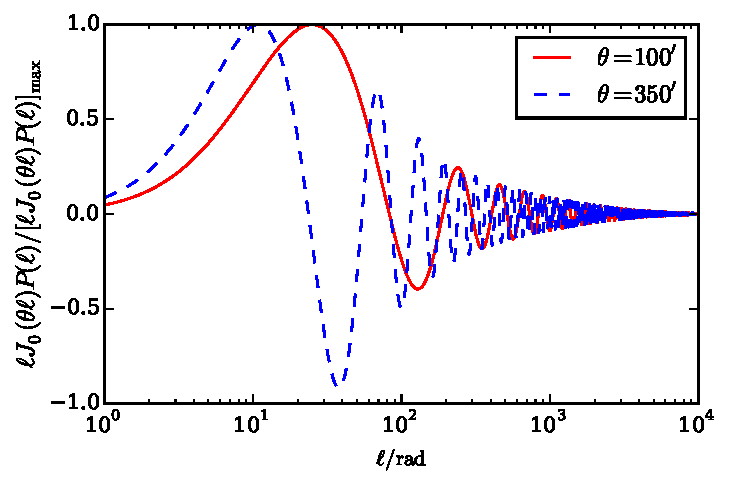
\includegraphics[width=0.31\textwidth]{figures/IntegKsip.pdf} &
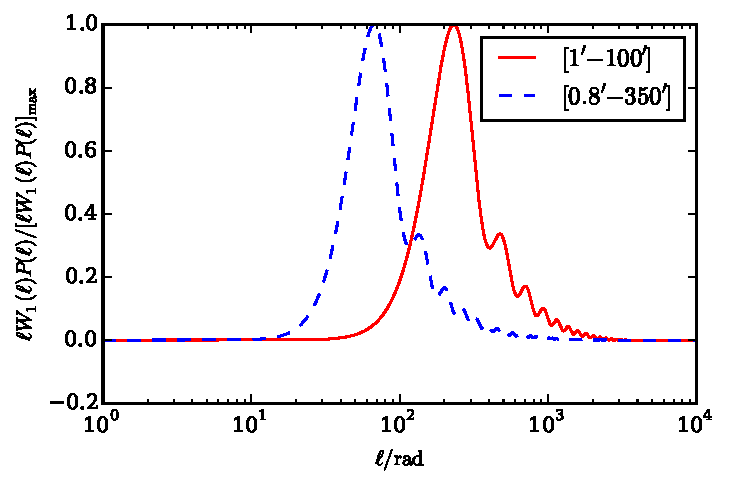
\includegraphics[width=0.31\textwidth]{figures/IntegCOSEBIs.pdf} &
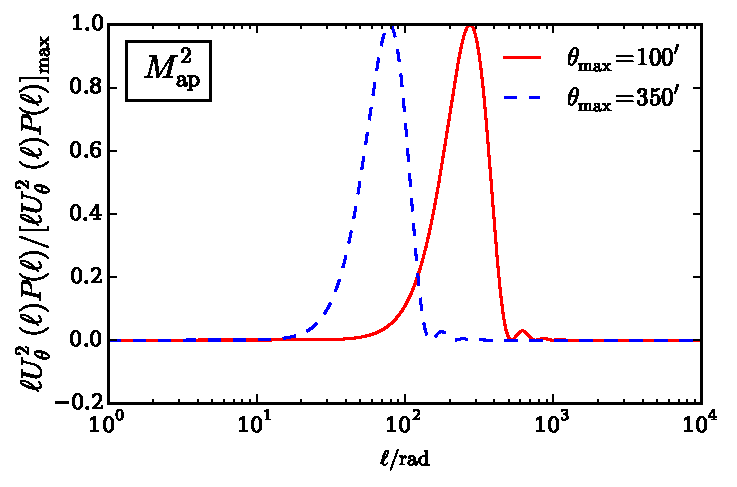
\includegraphics[width=0.31\textwidth]{figures/IntegMap.pdf}
\end{tabular}
\caption{ \label{fig:filters}. Integrand of $\xi_+$, $E_1$ (E-COSEBIs) and $M^2_{\rm ap}$, respectively.
Two cases are shown for each statistic as listed in each caption.
For the aperture mass statistic $\theta_{\rm max}=2\theta$ is shown. 
Note that higher order COSEBIs modes generally probe larger $\ell$-modes, hence here we only show the lowest mode $E_1$. All values are normalized with respect to their maximum value. 
}
\end{center}
\end{figure}


\subsection{On the Validation of Methods on Simulations}
It is discussed in \citet{kitching/etal:2016} that the validation of cosmic shear estimators on mock catalogues could also be affected by the approximations they investigate.  We agree that a full sky mock should be compared to a full curved sky non-Limber prediction.  It is then suggested, however, that the discrepancies already reported between existing mocks and the predictions could be attributed to these approximations, as opposed to a finite box effect \citep{kiessling/etal:2011, harnois-deraps/etal:2012, harnois-deraps/vanwaerbeke:2015}.  Going beyond flat sky and Limber could improve the agreement, however this cannot explain the results of \citet{harnois-deraps/vanwaerbeke:2015} who demonstrate that the large scale under-estimation of power varies with the simulation box size. This volume effect was verified by comparing explicitly the $\xi_+$ statistic at large angular scales between simulation volumes with box sides = 147Mpc/h and 515Mpc/h \citep[see Fig. 5 in][]{harnois-deraps/vanwaerbeke:2015}. The increase of power loss with decreasing box size was shown to be fully-modelled by excluding the super-box $k$-modes in the Limber predictions, something that the approximations discussed in \citet{kitching/etal:2016} would be unable to explain.

We note that any future comparison of mock data with full curved sky non-Limber predictions would place requirements on the input weak lensing simulations.  Many work with parallel plane mass-sheets as opposed to curved sky mass-sheets and at large angles these two approaches differ, regardless of the box size. 

\subsection{On the application to CMB lensing}
\citet{kitching/etal:2016} argue that their correction to the Limber and flat sky approximations would also affect predictions involving the shear and convergence cross-spectrum, such that CMB lensing - galaxy lensing cross-correlation should include a pre-term $ [\ell(\ell+1)]^2/(\ell+ 0.5)^4.$.   We have verified that this term would have negligible impact on the current measurements, given the relatively low signal to noise ratio. For example, most measurements \citep{hand/etal:2015, liu/hill:2015, kirk/etal:2016,harnois-deraps/etal:2016} are carried over angular multipoles in the range $\ell \in [20-2000]$, and are organized in $\sim$ five bins. The size of the pre-term $ [(\ell(\ell+1))^2]/(\ell+ 0.5)^4.$, averaged over the first bin, is of the order of 2\%, and then becomes sub-percent for all other bins. In comparison, the size of the statistical error bars are of the order 25-35\% with additional uncertainty due to photometric redshifts (10-15\%) and intrinsic galaxy alignments (10-15\%).





